\chapter{Introducción}
La realización de este trabajo de fin de grado se sitúa en el CTT, en concreto en el seno del grupo de investigación de realidad virtual, dentro de la Universidad de Granada. Dicho equipo desarrolla tareas de investigación con dispositivos de VR y AR y colabora en el proyecto de EuroFusion realizando la simulación y automatización de distintos procesos que tendrán lugar en el citado proyecto: IFMIF-DONES, a través de la manipulación de brazos robóticos.

En este primer capítulo introductorio desarrollaremos, de forma general, una contextualización del marco del proyecto en que nos hallamos y el ámbito en que este tiene lugar. Adicionalmente, conoceremos en las subsecciones contenidas el aliciente de la realización de este trabajo y el propósito que lo engloba, describiendo las tareas que precisarán de las tecnologías de las que haremos uso en nuestra investigación.

A continuación, se exponen los objetivos que se persiguen y propusieron, junto a la especificación del desarrollo del trabajo realizado, tanto en lo que a materiales utilizados como al tiempo que ha tomado su realización respecta.

Finalmente, en la sección que cierra este capítulo, se describen además los costos entrañados por este estudio de forma estimada tomando en cuenta tanto los recursos humanos invertidos así como los dispositivos y servicios. 

\vfill

\section{Sistemas Teleoperados}
Desde sus orígenes, el ser humano trata de adaptarse a su entorno, a la par que trata de tener una mayor comprensión de la naturaleza para poder aprovechar los recursos de esta en su favor, logrando así progresar. Parte de este trabajo consiste a su vez en adaptar el ambiente en que este habita para poder establecer un refugio y, ya asentado, poder sobrevivir junto al medio.

Pero la curiosidad con la que nacemos y la aspiración de comprender todo lo que nos rodea, incluso los rincones más recónditos, nos empuja a ingeniar métodos para ir más allá. Es entonces, en el momento en que nuestra anatomía no nos permite seguir avanzando, cuando tratamos de, con nuestro ingenio, forjar procedimientos que nos capaciten para poder dar un paso más y poder continuar conociendo el mundo que nos rodea.

Bajo estas premisas, podríamos pensar en cómo nuestra raza ha conquistado la tierra, los mares y se lanza ahora a la conquista del espacio exterior. Para ello, como se citó anteriormente, ideamos maneras de acceder a los lugares que nuestras condiciones de vida no nos permiten utilizando herramientas que puedan contribuir en el antedicho trabajo de estudio del mundo y el cosmos que nos sirvan de apoyo, como lo son los robots.

La idea de poder asistir y contemplar aquellos lugares inhóspitos jamás visitados es algo que nos fascina y a su vez una idea que cada vez tenemos más cerca. Es por ello que trabajamos en tecnologías como la robótica, que nos permiten tener ojos, oídos e incluso tacto donde no lo tenemos. En este punto, surge el concepto de telerrobótica, un área de la propia robótica que estudia el control de autómatas de forma remota, y es aquí donde aparece el término que titula esta sección: la teleoperación.

Podemos reseñar este concepto, como el designio técnico para  la utilización y control de una máquina, sistema, robot o vehículo de forma telemática. Esta metodología de control consiste regularmente en el uso de cualquiera de los citados instrumentos, que tendrán sensores y actuadores incluidos, por parte de un operario; que comanda a distancia su comportamiento desde un punto desde el que es seguro trabajar. Los manipuladores, que controlarán los dispositivos finales que trabajarán in situ, son generalmente adiestrados antes de realizar las tareas asignadas  con simulaciones y en ambientes controlados para no dañar los equipos reales de trabajo además de tener un tiempo de práctica y aprendizaje \cite{5}. 

A su vez, las actividades ejercidas por los operarios que se dedican al control de equipos a distancia son variopintas y dependen en gran medida del objetivo a cumplir. En líneas generales, los equipos se diseñan y adaptan para cumplir con propósitos específicos, dependiendo siempre de la complejidad de la tarea; aunque existen en el mercado cantidad de soluciones genéricas que serían suficientes para ciertos cometidos. Algunos ejemplos de ello podemos encontrarlos en las grúas situadas en puertos marítimos, para el manejo de logística, e incluso en la propia Estación Espacial Internacional con sus conocidos Canadarm y Canadarm2, \ref{fig:canadarm}.

Este último es parte de la aportación de Canadá al proyecto ISS. Con una longitud de  17.59 m, este gran brazo robótico es utilizado para realizar tareas de mantenimiento en la estación, traslado de equipos y suministros o asistencia en el aterrizaje de vehículos visitantes siendo controlado por los astronautas a bordo o desde tierra en las sedes de la CASA o la propia NASA \cite{90}. 

\begin{figure}[hbt]
    \centering
    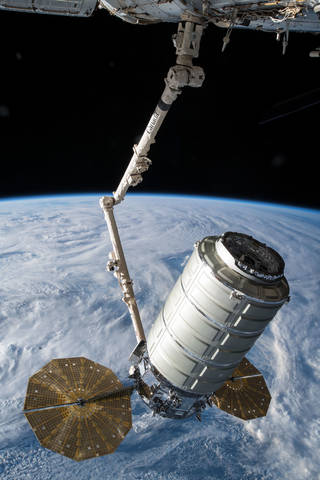
\includegraphics[width=0.25\textwidth]{imagenes/canadarm2.jpg}
    \caption{\cite{81}}
    \label{fig:canadarm}
\end{figure}

Sin embargo, en la mayoría de los casos de uso complejos, la información que estos reciben a través de los receptores no es suficiente para cumplir de manera adecuada con las tareas asignadas, ya que existen restricciones que suponen barreras infranqueables para completar ciertas labores, sean impuestas por el entorno o por la naturaleza de la propia actividad a desempeñar. Es por ello que se sigue esta línea de investigación, para hacer la experiencia del usuario que controla telemáticamente sea más inmersiva y similar a la presencia en el espacio de trabajo. 


\section{Tecnologías inmersivas}
Podemos describir la percepción de nuestro entorno como el producto de la capacidad de nuestra mente para interpretar y poner orden a la ingente cantidad de información que recibe a través de los sentidos. La forma en que se transforman los estímulos recibidos como distintas manifestaciones de reacciones químicas y eléctricas a través del sistema nervioso, y cómo nuestro cerebro ordena ese caos para darle un sentido racional es asombrosa.

Con el brutal aumento en la potencia de cómputo en los últimos años y gracias a la gran apuesta que se ha hecho por las nuevas tecnologías, los resultados conseguidos para la simulación de escenarios ficticios son, en algunos casos, prácticamente indistinguibles de la realidad. Es por ello, que el uso de la realidad virtual, por ejemplo, para recrear parajes, experiencias y sensaciones está cada vez más extendido y ve su auge en nuestros días.

Podemos definir las tecnologías inmersivas, de forma genérica, como la aplicación de los tipos existentes dentro de esta disciplina (VR, AR y MR), usados en conjunción con otros métodos con capacidades multisensoriales, para la intensificación de la experiencia que se trata de simular, como haremos con la retroalimentación háptica \cite{91}. En consecuencia, es ostensible el potencial de esta modalidad para su aplicación en áreas como el desarrollo industrial, la educación, el diseño, etc.

Consecuentemente, consideramos que esta tecnología posee un alto valor para su integración en el marco de trabajo establecido para nuestro proyecto. Así pues, la coordinación de los métodos de teleoperación, junto a la información percibida por el operador del entorno del dispositivo controlado, gracias a los métodos de inmersión, pueden hacer que la experiencia sea satisfactoriamente cercana a la actuación presencial.

\section{Marco de trabajo: IFMIF-DONES}

La evolución del ser humano como sociedad y el consumo de energía en su desarrollo han estado profundamente ligados en el curso de la historia. Tanto es así que incluso fueron propuestos métodos tales como la escala de kardashov, por el astrofísico ruso Nikolái Kardashov \cite{92}, para medir la evolución tecnológica de una civilización en relación a la cantidad de recursos energéticos que esta es capaz de aprovechar de su entorno.

Dicho esto, y congruentemente con lo comentado, es evidente que la dirección en la que se dirige nuestro progreso como sociedad está estrechamente relacionado de forma directa con la forma en que obtenemos y hacemos uso de la energía, y es por ello que se trata en todo momento de encontrar formas efectivas y eficientes tanto de emplearla como de obtenerla, intentando mejorar los procedimientos existentes. 

Actualmente, las principales fuentes de energía utilizadas en todo el mundo derivan de los combustibles fósiles, figura \ref{fig:energy_graph}, energías que no son renovables y cuyas reservas serán agotadas en las décadas venideras. De igual modo, este tipo de comburentes emiten grandes cantidades de gases de efecto invernadero al ser consumidos, y este factor, sumado al cambio climático, cuyos efectos ya son palpables en todo el globo, constituyen una combinación fatal.

\begin{figure}[hbt]
    \centering
    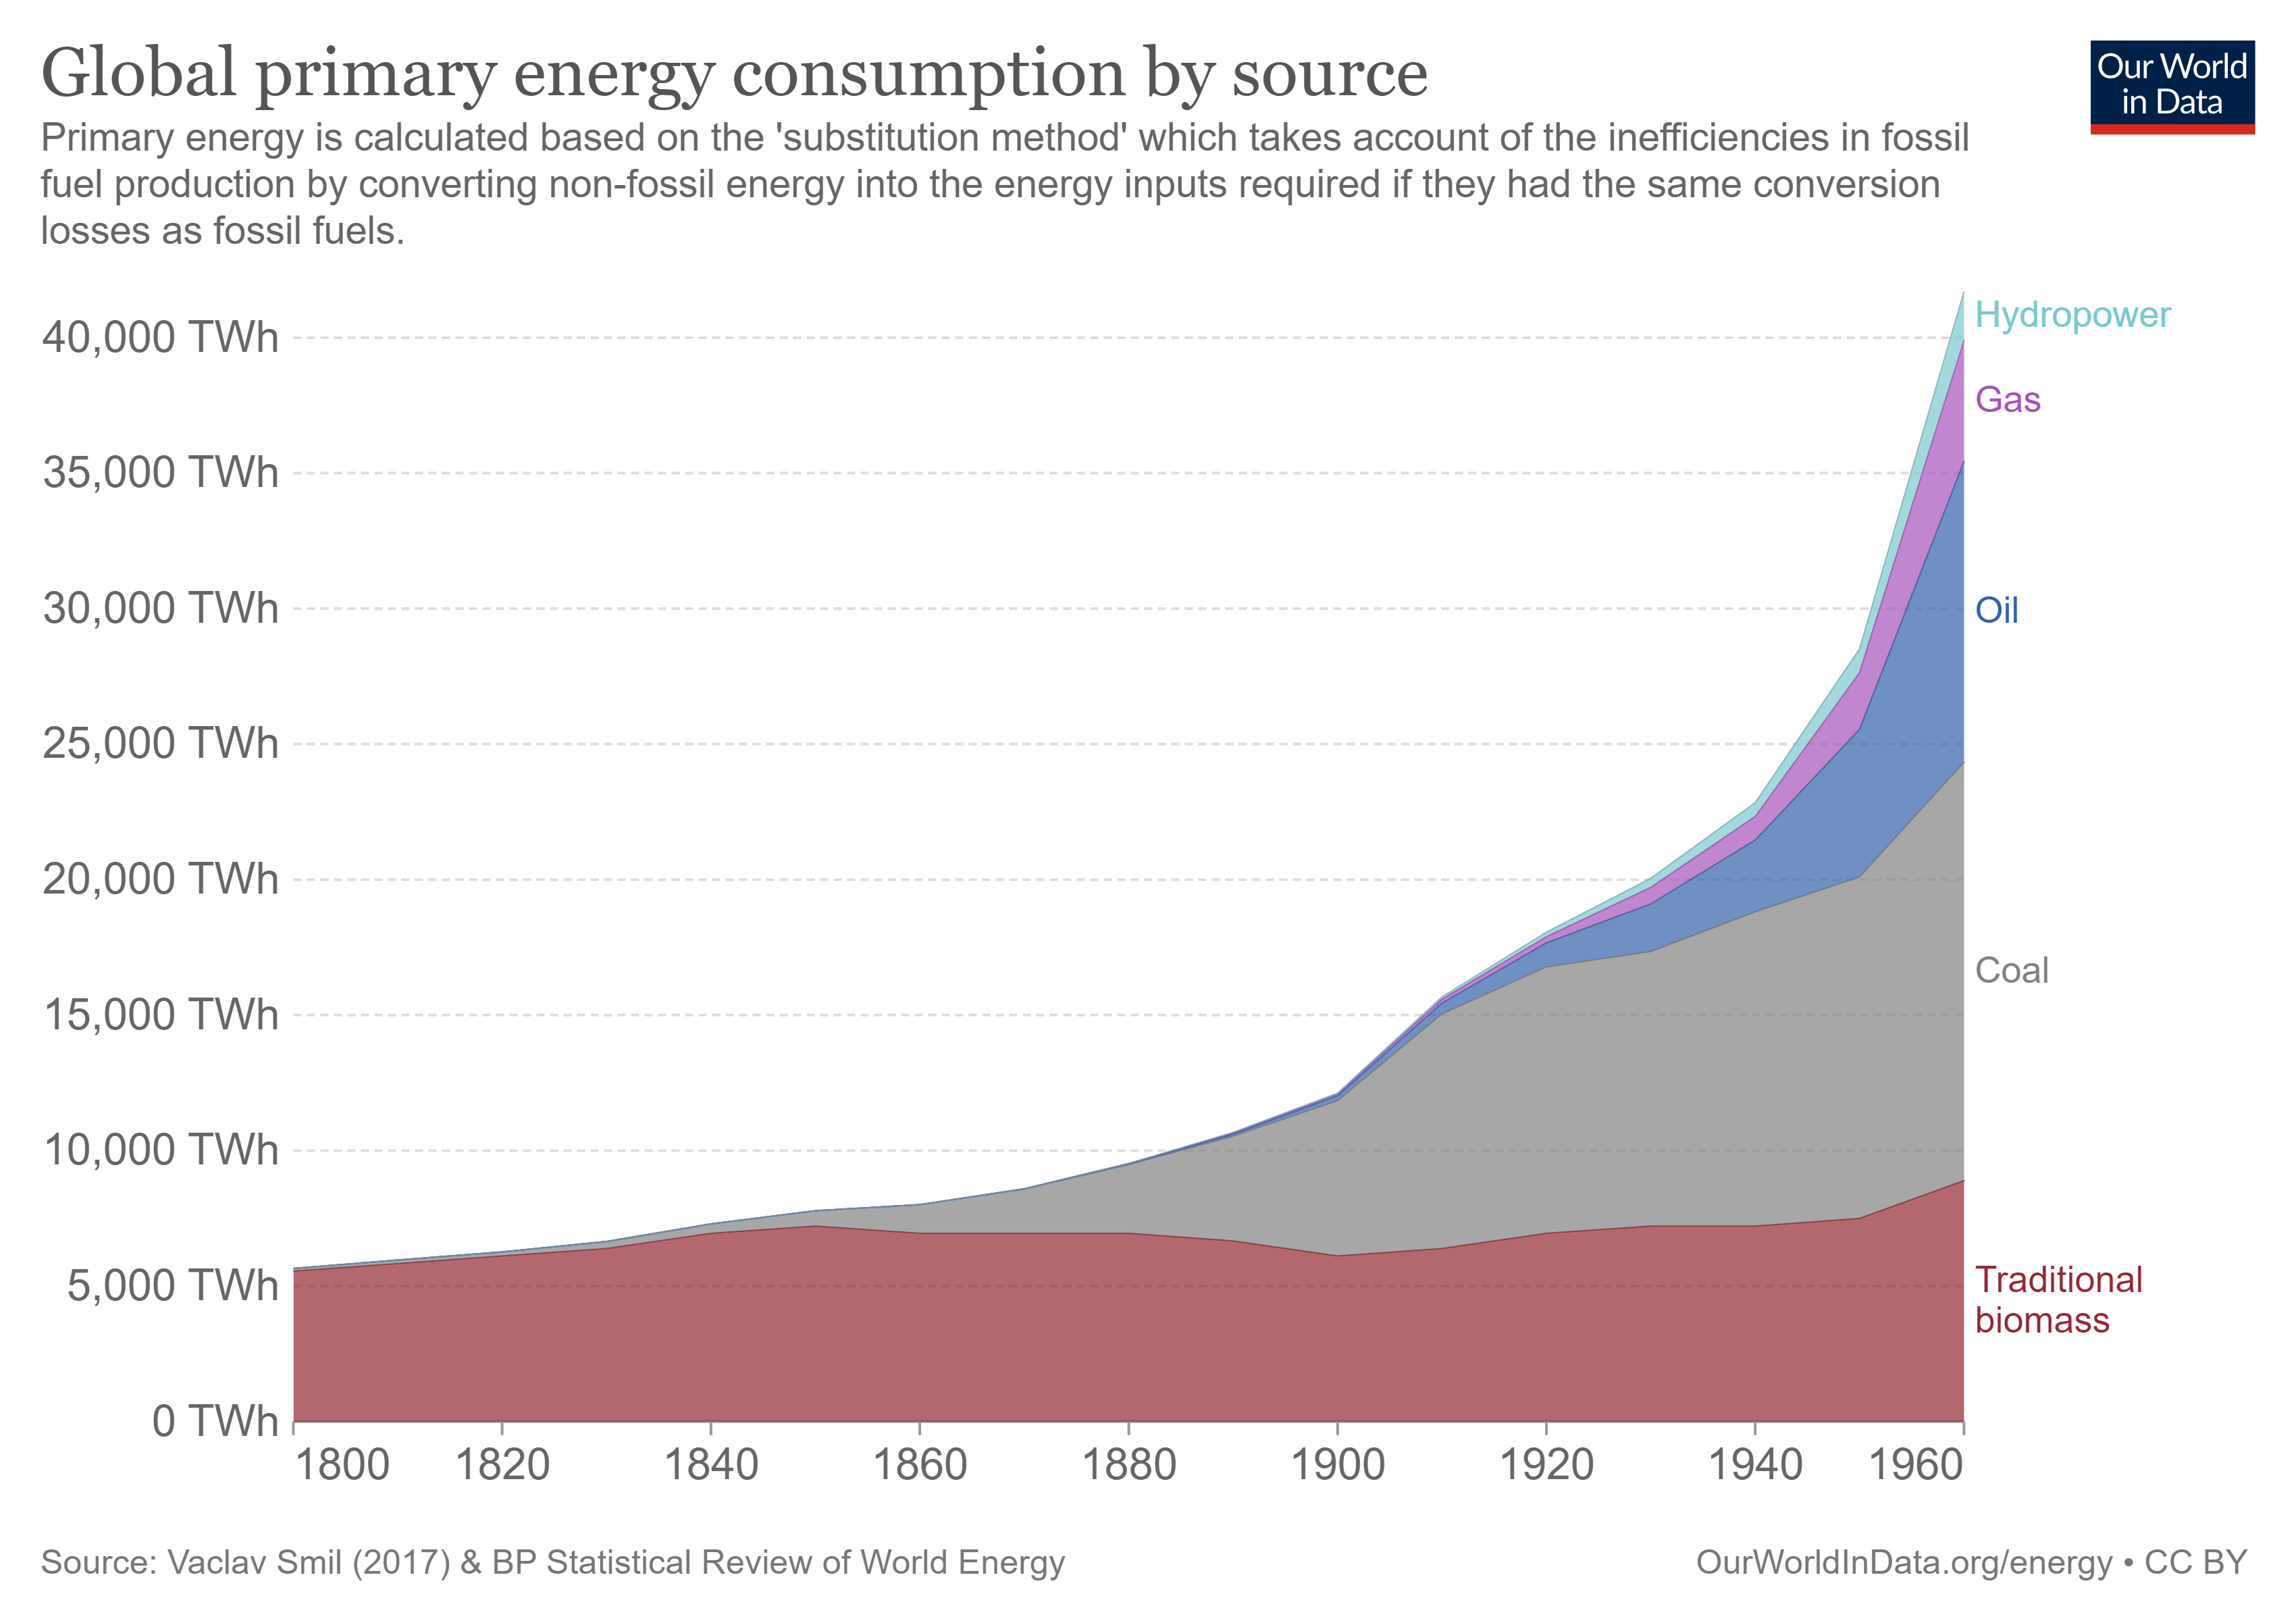
\includegraphics[width=0.75\textwidth]{imagenes/global-energy-substitution.png}
    \caption{\cite{82}}
    \label{fig:energy_graph}
\end{figure}


A ese respecto, se apuesta de forma unánime en todas las naciones por las energías de carácter renovable y con bajas o nulas emisiones para mitigar o reducir los citados efectos del calentamiento global, y es entre ellas que encontramos el motivo de realización de este y otros muchos proyectos que contribuyen a la búsqueda de la obtención de energía a través de la Fusión Nuclear . 

Descrito el contexto que engloba a este estudio, el trabajo de investigación realizado tratará de realizar una aportación en el seno del programa IFMIF-DONES, que figura en la hoja de ruta para alcanzar reactores comerciales que puedan lograr las mencionadas reacciones nucleares.

En este caso, nos centraremos en el apoyo a las tareas de mantenimiento que tendrán lugar; que deberán realizarse en gran parte de los casos a distancia, al menos en las inmediaciones del reactor. Las razones de ello, como cabe esperar, son principalmente las grandes corrientes de radiación que circulan en algunas zonas de las instalaciones, por los isótopos radiactivos de los materiales utilizados en el proceso de fusión y la gran cantidad de neutrones rápidos que se desprenden de las propias reacciones, haciendo de este un ambiente extremadamente nocivo para el ser humano.

\section{Objetivos Planteados}
Los objetivos, como metas que pretenden alcanzarse, definen en esencia las acciones básicas que se realizarán en el marco de un proyecto para, en efecto, trazar una hoja de ruta. En nuestro caso podemos asumir el objetivo general y su motivación como  aclarados en las secciones precedentes.

Como objetivos específicos definiremos algunas tareas que son de obligada consecución para la completa cobertura de los requerimientos que suponemos como básicos y necesarios.

\begin{itemize}
    \item Simular de forma correcta el robot Baxter en Unity para poder trabajar con el mismo en la simulación llevada a cabo. 
    \item Conseguir conectar el dispositivo háptico con Unity y acto seguido tratar de realizar una correspondencia entre ambos robots para lograr el control de Baxter a través del dispositivo háptico.
    \item Tratar de hacer uso de las extensiones existentes para el control del feedback háptico, y en caso de no ser viable investigar la documentación disponible para el artefacto para desarrollar una implementación propia del mismo.
    \item Refinada la reacción al contacto con objetos implementar la posibilidad de agarrarlos y desarrollar la respectiva sensación táctil asociada.
    \item Realizar test de las funcionalidades implementadas para revisar su correcto funcionamiento y rendimiento además de tomar datos acerca del progreso conseguido para realizar gráficas e informes.
    \item Trasladar las posiciones calculadas en las que debe situarse el robot controlado al Baxter real y testear su correcto funcionamiento.
\end{itemize}

\section{Planificación del Proyecto}
El proceso de toma de decisiones previo a la realización de un proyecto, teniendo en cuenta parámetros como el tiempo disponible, los recursos a nuestro alcance y los posibles contratiempos, es una práctica obligada en la correcta ejecución de las tareas que conciernen al campo de la ingeniería y en general a la ciencia. Es por ello que se exponen en esta sección las distintas etapas que se planificaron y por las que ha discurrido nuestro proyecto.

En el diagrama realizado, figura \ref{fig:diagrama_gantt}, podemos observar una progresión clara por distintas fases hasta completar la puesta en marcha y documentación de este proyecto. En principio, podemos asociar a cada una de las semanas de trabajo una media de 30 horas semanales, con lo que la realización completa de este TFG ha tomado alrededor de 330 horas. La idea de planificación inicial se fundamentó en la realización de una nueva tarea cada semana, lo cual se ha intentado respetar al máximo en la medida de lo posible.


\begin{figure}[hbt]
    \centering
    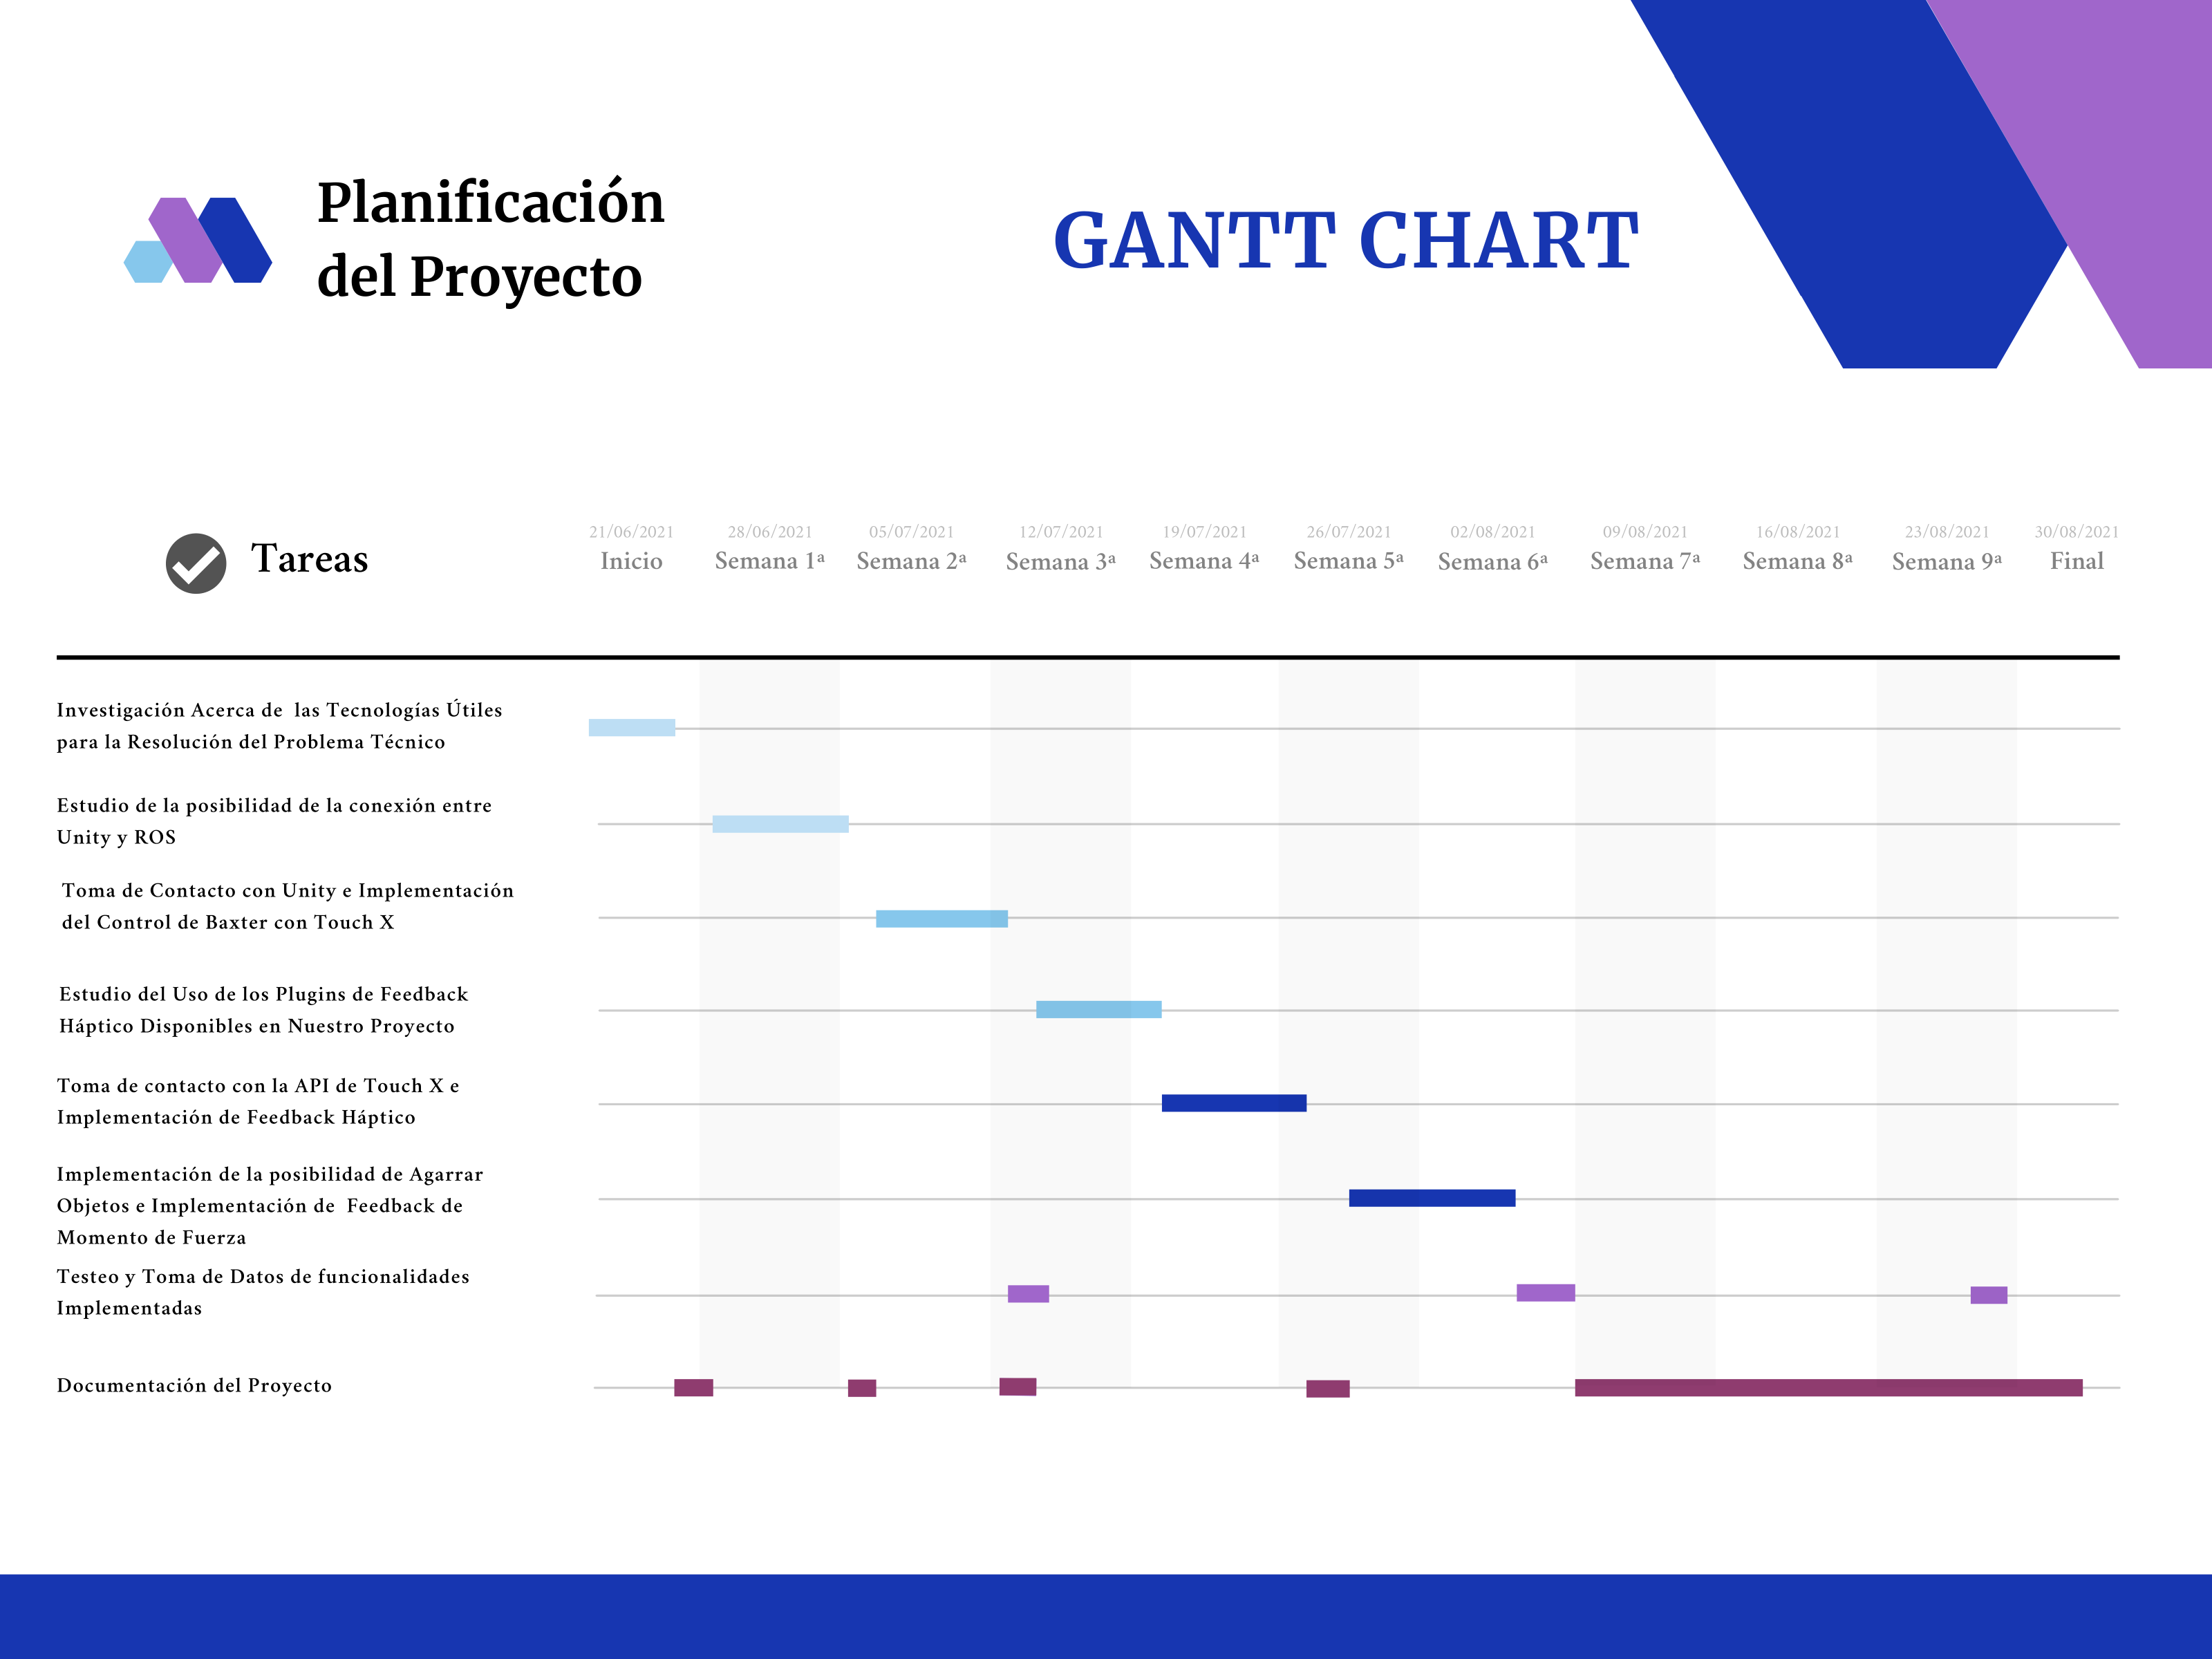
\includegraphics[width=1\textwidth]{imagenes/DiagramaGantt.png}
    \caption{}
    \label{fig:diagrama_gantt}
\end{figure}

En primera instancia, se realizaron tareas de búsqueda acerca de las tecnologías disponibles para la realización del proyecto y el análisis de ventajas e inconvenientes de cada una de las opciones posibles. A tal efecto, la combinación de las tecnologías elegidas resulta  bastante sinérgica, haciendo que la integración de las unas con las otras sea sencilla y eficiente. Adicionalmente, los compañeros en el grupo de investigación en el que este proyecto tuvo cabida trabajan actualmente con algunas de ellas, resultando más sencilla, en caso de ser útil, la integración de la investigación realizada con el resto del proyecto. 

Tras ello, tratamos de realizar la conexión entre Baxter y Unity, explorado así las distintas vías para la consecución de este objetivo, como las extensiones disponibles de las que podíamos hacer uso. Sin embargo, en el momento en que hubimos recabado toda la información necesaria para comenzar la programación, decidimos redistribuir el tiempo, tratando de dedicar una mayor cantidad de horas al feedback háptico y su implementación. Esta decisión se tomó en base a que esta era una característica crucial, considerando pues como opcional esta comentada actividad, ya que la simulación resulta suficiente para nuestra investigación.


A continuación procedimos a tomar contacto con Unity, su entorno y el scripting en C\#. Esta tarea no supuso un impedimento, ya que es conocida la programación orientada a objetos por nuestra parte y se ha trabajado  en ocasiones anteriores con lenguajes derivados de C, con lo que se comenzó con la implementación del control de Baxter en la simulación a través del dispositivo háptico realizando una correspondencia de las articulaciones en ambos robots.

Tras ello, se trató de comprender el funcionamiento de los plugins que materializan el feedback háptico en consecuencia a la simulación para usarlos junto a la parte ya diseñada, pero el resultado fue infructuoso. Se invirtió alrededor de una semana en tratar de llevar a efecto esta solución, ya que resultaba bastante prometedora, pero el uso de los complementos diseñados junto al control implementado por nuestra parte fue imposible. 

En vista a los resultados, se procedió al estudio de la documentación disponible por parte del dispositivo háptico para desarrollar una serie de funciones y scripts que, haciendo uso de la API, gestionan y controlan todo lo que respecta a la monitorización y el manejo del susodicho robot. Esta etapa resultó complicada, y ha sufrido modificaciones hasta el último momento, ya que la decisión final de implementación ha sido fruto del testeo de los distintos métodos existentes para realizar tareas concretas.

Conocida la interfaz de acceso a la máquina, se prosiguió con la simulación de los efectos de gravedad y momento o torque; dos características esenciales para que la sensación táctil se torne lo más fiel a la realidad posible. Para ello se hizo uso de física básica, calculando las medidas de velocidad, aceleración, masa y torque a través de los datos proporcionados por Unity.

Finalmente, en lo que a la toma de medidas y realización de test respecta, podemos ver como en el diagrama se refleja la dedicación de parte del tiempo disponible al final de cada etapa de desarrollo de nuevas características para ello. Tras su puesta en marcha, cada una de las funcionalidades debía ser testeada y ajustada para que el resultado esperado además de ser objetivo resulte agradable y natural para el usuario final.

\section{Estimación de Costos}

La gestión y estimación de costes constituyen una actividad esencial para asignar y controlar exactamente a qué partes se destina el presupuesto disponible para un proyecto. Ello permite a las entidades involucradas conocer de antemano 	la distribución del capital utilizable en el mismo y anticiparse a los gastos que puedan surgir como imprevistos.

Procederemos pues, a realizar un análisis de los equipos y servicios utilizados y a realizar el cálculo de un coste estimado \ref{tab:estimacion_de_costos}.

\bigskip
\bigskip
\bigskip
\bigskip
\bigskip
\bigskip
\bigskip
\bigskip
\bigskip
\bigskip

\begin{table}[hbt]
    \centering
    \begin{tabular}{l p{0.3\linewidth} c c}
        \specialrule{.1em}{.05em}{.05em} 
        \textbf{Servicio} & \textbf{Uso} & \textbf{Unidad} & \textbf{Coste} \\
        \specialrule{.1em}{.05em}{.05em}
        Computador & Realización de tareas de renderizado y simulación & 1 & 277.77 \euro \\
        Dispositivo Háptico & Necesario para el control de Baxter y para proporcionar el feedback háptico & 1 & 8440.00 \euro \\
        Investigador & - & 1 & 554.60 \euro \\
        Licencia de Unity & Entorno de simulación y realidad virtual & 1 & 508.50 \euro \\
        \specialrule{.1em}{.05em}{.05em}
    \end{tabular}
    \caption{Análisis de costos}
    \label{tab:estimacion_de_costos}
\end{table}

El cálculo del coste del computador ha sido llevado a cabo considerando un coste del equipo de 2500\euro  y un uso del mismo en un periodo de 4 meses. De este modo, estimando una amortización de 3 años, el coste valorado es de 277,77\euro.

Para el sueldo del investigador se tiene en cuenta un salario base de 2500\euro, a lo que hay que sumar un 33\% por los costes asociados a la seguridad social en un contrato de 1800 horas anuales. En este caso estimamos unas 300 horas de trabajo, que son las supuestamente destinadas al trabajo de final de grado, con lo que tasamos un importe de 554.60\euro.

En el caso de la licencia para el uso de Unity consideramos que el plan utilizado sería el de Unity Pro, con un coste total anual aproximado de 1,525.51\euro. Sabiendo esto, y considerando un uso por 4 meses, estimamos un importe a pagar de 508.50\euro.
